\section{Hyperdimensional embeddings on the level of amino acids}
\subsection*{Encoding biological information into a vector}
Currently, in most of the research in hyperdimensional computing, there is an emphasis on creating and assigning hyperdimensional vectors fully randomly to certain concepts. This is useful for optimizing speed and efficiency and is not a problem for many cases such as natural language processing, where it is usually assumed that a letter does not have varying degrees of similarities to other letters in the alphabet. For protein language modeling, however, this assumption is not valid since some amino acids are chemically more similar to each other than to others, but also in an evolutionary sense. It is not uncommon to spot substitutions on the level of amino acids within the same proteins between different species and to barely notice changes in structure and function.

To account for this, we tried to encode the biological information of amino acids into HDVs by extending existing embeddings into hyperdimensionality and comparing these to baseline random hypervectors. To assess this, the vectors for each amino acids are reduced in dimensionality \textit{via} PCA into 2 dimensions and then plotted as seen in figures~\ref{fig:AArand} and~\ref{fig:AAesm}. At first glance, there is not much to spot. Yet, there is significantly more variance encoded into the first two principal components of the ESM embeddings compared to the random vectors, meaning that there should be a significant amount of similarity encoded into the hyperdimensional vectors. This may be shown more clearly when used and compared in real-world problems.
\begin{figure}[H]
    \centering
    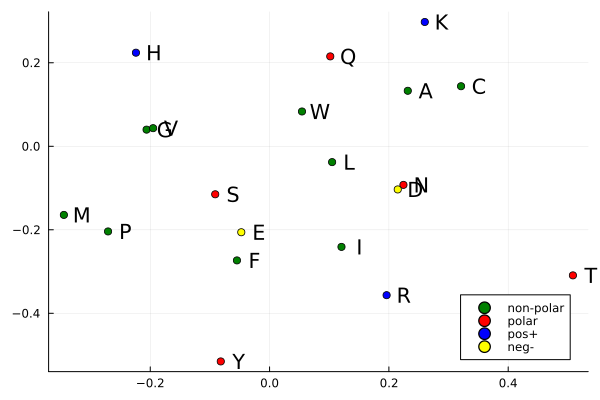
\includegraphics[scale = 0.5]{random_emb}
    \caption{Scatter-plot of the first two principal components of random hyperdimensional vectors assigned to amino acids to set a baseline level. These PCs account for roughly 10.5 \% of the total variance. The amino acids are annotated and colored based on their chemical property of polarity. This plot can look completely different depending on the run.}\label{fig:AArand}
\end{figure}

\begin{figure}[H]
    \centering
    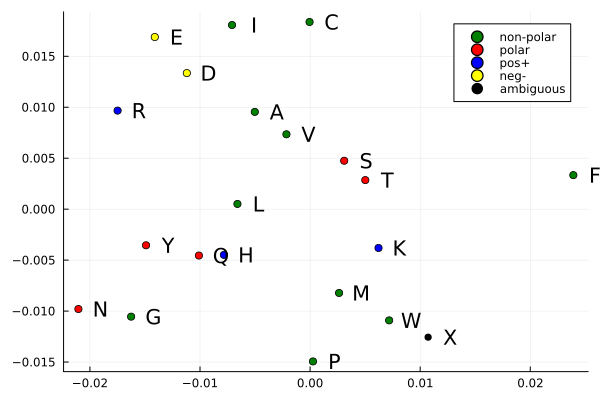
\includegraphics[scale = 0.5]{esm_emb}
    \caption{Scatter-plot of the first two principal components of ESM embeddings extended into hyperdimensionality. These PCs account for roughly 22 \% of the total variance. The amino acids are annotated and colored based on their chemical property of polarity.}\label{fig:AAesm}
\end{figure}

\subsection*{Encoding interactions of a residue's neighborhood into a vector}
State-of-the-art protein language models have the ability to gather information on long-range dependencies around a single amino acid and encode this information into neural networks and in embeddings. To investigate the possibilities of developing embeddings on the level of amino acids, we propose a novel encoding technique within the hyperdimensional computing framework. It encodes interactions of a given amino acid in a sequence to other amino acids in its neighborhood for a predetermined range. This method thus tries to learn information about an amino acid within a sequence in an unsupervised manner.
\begin{figure}[H]
    \centering
    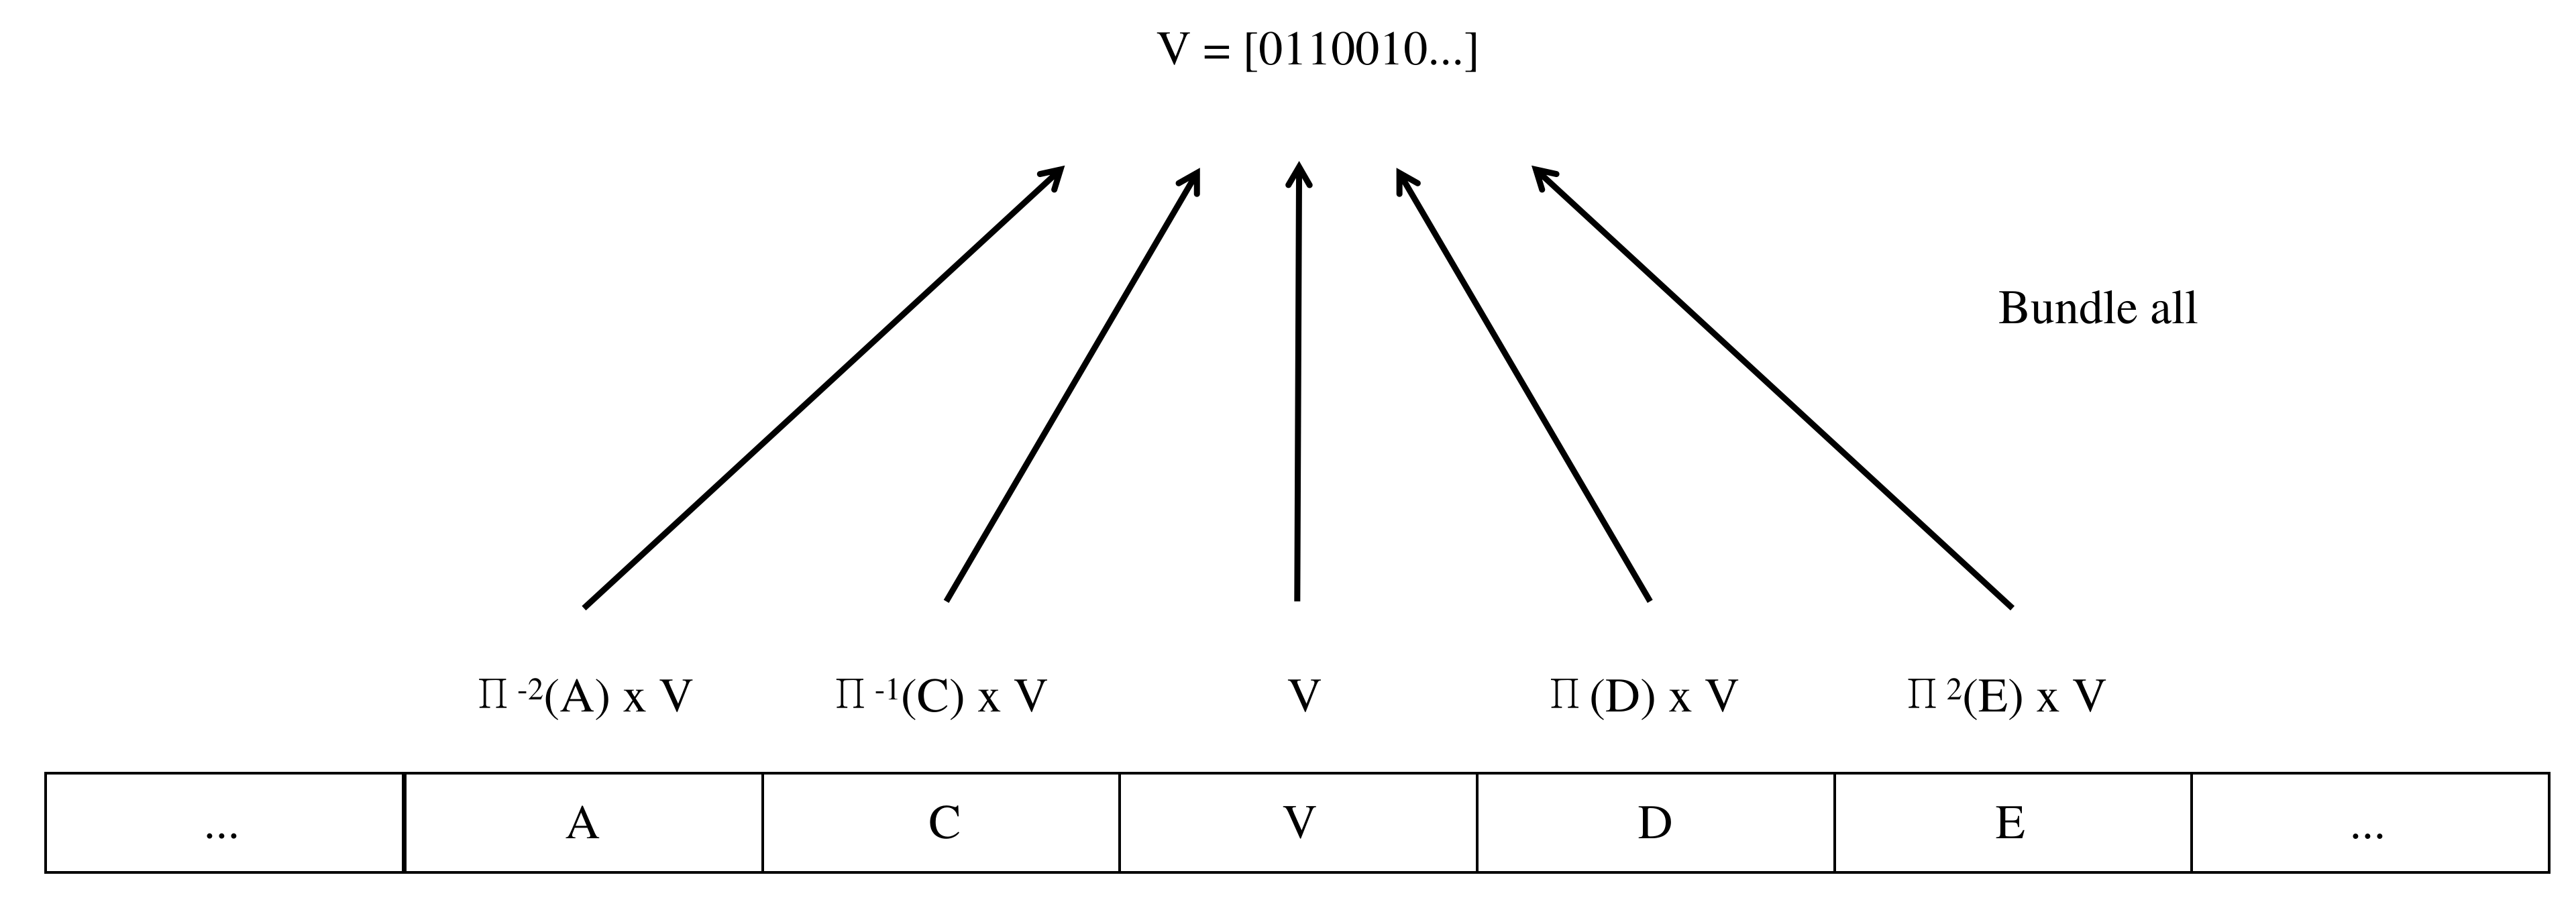
\includegraphics[scale = 0.15]{transformerlike}
    \caption{A simple demonstration of our amino acid encoder. It considers an amino acid and all amino acids in a predetermined distance (here k = 2). It produces all possible interactions of the central amino acid in the window by binding and then bundles all the pairwise interactions into one hyperdimensional vector that represents the central amino acid.}
    \label{fig:AAtr}
\end{figure}

Windows of $k = 4$ and $k = 50$ were considered for illustration purposes in figures \ref{fig:AAtr4} and \ref{fig:AAtr50}. Every single residue in the human reference proteome was encoded with information within the k-range window and an average vector was made for every amino acid. For all 20591 peptides in the reference proteome, this procedure took only 3 hours for $k = 4$, but upwards to 20 hours for $k = 50$ on a high-performance computing cluster (HPC). At first glance, the charged amino acids seem to be grouped vertically (PC 2), roughly dividing the polar and non-polar amino acids, albeit slightly more pronounced for $k = 50$. MORE TO ADD LATER WHEN TRIED WITH FULLY RANDOM VECTORS: Also interesting, the starting ESM embeddings are extended into hyperdimensionality in a random manner, so to see similar groupings in the PCA plots indicates that the first four amino acids before and after a residue are the most crucial.

\begin{figure}[H]
    \centering
    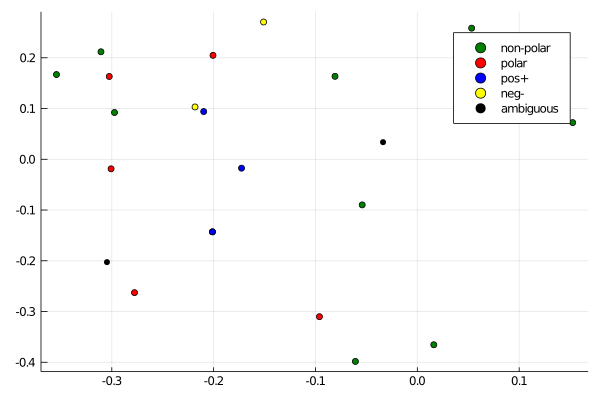
\includegraphics[scale = 0.5]{4tr_emb}
    \caption{Scatter-plot of the first two principal components of the average amino acid HDVs with neighborhood-information of $k = 4$ encoded, trained on the human reference proteome. These PCs account for roughly 21 \% of the total variance. The amino acids are annotated and colored based on their chemical property of polarity.}
    \label{fig:AAtr4}
\end{figure}

\begin{figure}[H]
    \centering
    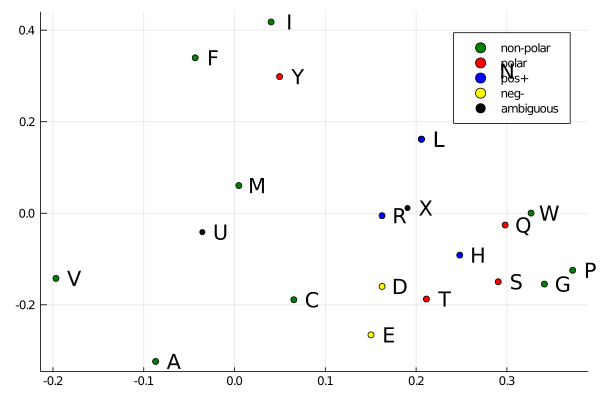
\includegraphics[scale = 0.5]{50tr_emb}
    \caption{Scatter-plot of the first two principal components of the average amino acid HDVs with neighborhood-information of $k = 50$ encoded, trained on the human reference proteome. These PCs account for roughly 21 \% of the total variance. The amino acids are annotated and colored based on their chemical property of polarity.}
    \label{fig:AAtr50}
\end{figure}